\section{\bf Multisymplectic geometry}

\subsection{Basic definitions}
\begin{frame}
    \frametitle{Basic definitions I}
    \begin{definition} A \alert{multisymplectic manifold} of order $n$ is a pair $(M, \omega)$, where $M$
        is a smooth manifold, and $\omega$ is a closed $(n+1)-$form.
    \end{definition}
    An immediate example is the bundle of $n$-forms on a manifold $Q$. $$M:= \bigwedge^n T^\ast Q \xrightarrow{\tau} Q$$ has 
    a canonical $n$-form, 
    $$\Theta|_{\alpha}(v_1, \dots, v_n) := \alpha(\tau_\ast v_1, \dots, \tau_\ast v_n)$$ and
    $$\Omega := - d  \Theta$$ defines a multisymplectic structure on $M$. 
\end{frame}

\begin{frame}
    \frametitle{Basic definitions II}
    \begin{Def} Let $(M, \omega)$ be a multisymplectic manifold of order $n$. A $q$-multivector field $U$ on $M$ ($q \leq n$) is
        called \alert{Hamiltonian} if $$\iota_U \omega = d \alpha,$$ for certain $(n - q)$-form $\alpha$, which will also
        be called \alert{Hamiltonian}.
    \end{Def}
    \begin{itemize}
        \item Top degree Hamiltonian multivector fields ($n$-multivector fields) represent \alert{solutions} to the variational problem, 
        $$\iota_U \omega  = dH, H \in C^ \infty(M).$$
        \item Hamiltonian vector fields $X \in \mathfrak{X}(M)$ are \alert{symmetries,} $\pounds_X \omega = 0$ and the corresponding
        $(n-1)-$form can be thought of as the \alert{Noether current} of the symmetry.
    \end{itemize}
\end{frame}

\subsection{Noether's Theorem}
\begin{frame}
    \frametitle{Noether's Theorem I}
    Given a Hamiltonian function $H$, and a top degree decomposable multivector field $U$ such that 
    $$\iota_U \omega = dH,$$ let $$j: \Sigma \hookrightarrow M$$ be an $n$-dimensional integral submanifold of $U$ (which can be thought of as a distribution).
    \begin{center}
        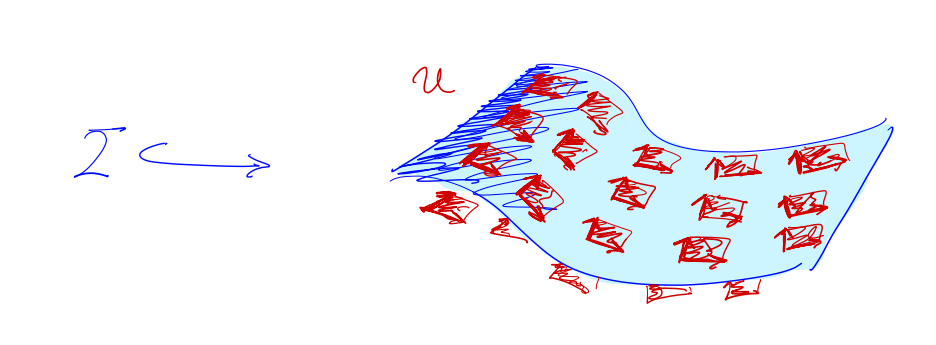
\includegraphics[height = 100pt]{Images/Multivector_variations.PNG}
    \end{center} 
\end{frame}

\begin{frame}
    \frametitle{Noether's Theorem II}
    \begin{theorem}Let $X$ be a Hamiltonian vector field and $\alpha$ the corresponding $(n-1)$-form (the current), $$\iota_X \omega = d \alpha.$$
        Then, if $X$ is a symmetry of $H$, that is, $$X(H) = 0,$$ $\alpha$ is a \alert{conserved current} on $\Sigma,$ this means
        $d(j^\ast \alpha) = 0.$
    \end{theorem}
    \begin{proof} Indeed,
        $$(d\alpha)(U) = \iota U \iota_X \Omega = (-1)^n \iota_X \iota_U \Omega = (-1)^n X(H) = 0.$$
    \end{proof}
\end{frame}

\begin{frame}
    \frametitle{Noether's Theorem III}
    \begin{center}
        {\large \bf What does \alert{conserved} means here?}
    \end{center}
    \begin{center}
        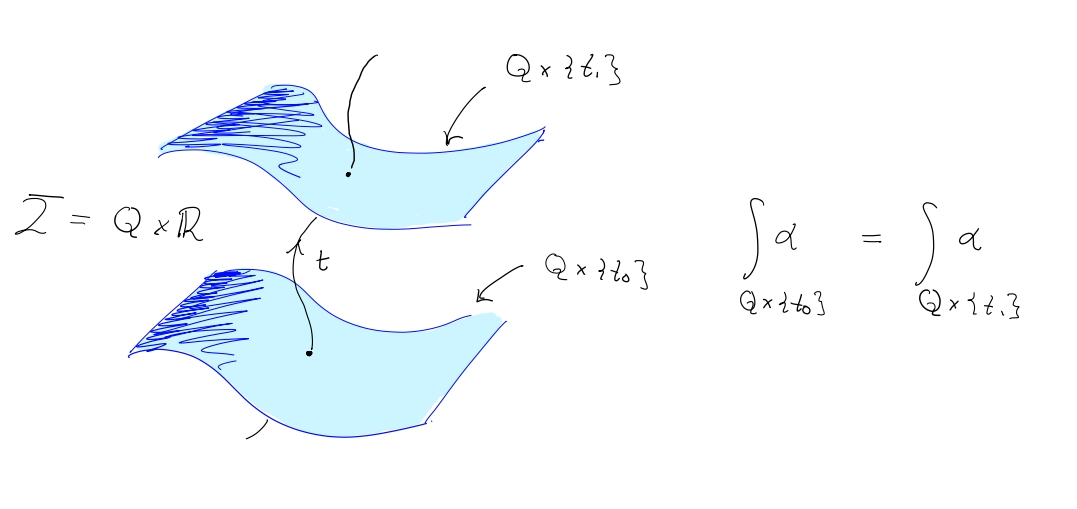
\includegraphics[width = 330 pt]{Images/Noether_current.PNG}
    \end{center}
\end{frame}

\begin{frame}
    \frametitle{Noether's Theorem IV}
    {\large \bf How can we obtain the corresponding current from the symmetry defined by $X$?}
    \begin{theorem} Let $(M, \omega)$ be an \alert{exact} multisymplectic manifold, that is, there exists a \alert{multisymplectic potential}
        $$\omega = - d \theta.$$ Then, if $X$ is a symmetry of $\theta$, $\pounds_X \theta = 0$ (and hence of $\omega$), $$\alpha := - \iota_X \theta$$
        is a current for $X$.
    \end{theorem}
    \begin{proof} Indeed, $$d \alpha = - d \iota_X \theta = - \iota_X d \theta = \iota_X \omega.$$
    \end{proof}
\end{frame}

\subsection{Brackets}
\begin{frame}
    \frametitle{Brackets I}
    \begin{proposition} Let $(M, \omega)$ be a multisymplectic manifold and $\alpha,$ $\beta$ be Hamiltonian forms,
        with Hamiltonian multivector fields, $X$, $Y$, respectively. Then $$\{\alpha, \beta\} := \iota_Y \iota_X \omega$$ is a Hamiltonian form. Its
        Hamiltonian multivector field is $-[X, Y]$ (the Schouten-Nijenhuis bracket).
    \end{proposition}

    \begin{definition}
        Define the \alert{Poisson bracket} of two Hamiltonian forms by $$\{\alpha, \beta\} := -(-1)^{(k - 1 -\operatorname{ord} \alpha )}\iota_Y \iota_X \omega,$$ which is again
        Hamiltonian by the previous proposition.
    \end{definition}
\end{frame}

\begin{frame}
    \frametitle{Brackets II}
    \begin{center}
        {\large \bf What are the properties that $\{\cdot, \cdot\}$ satisfies?}
    \end{center}
    If we define a new degree: $$\deg \alpha:= k -1 - \text{ord} \alpha,$$

    \begin{itemize}
        \item It is \alert{\textit{graded-skew-symmetric}}, that is, $$\{\alpha, \beta\} = (-1)^{\deg \alpha\deg \beta} \{\beta, \alpha\}.$$
        \item Its satisfies \alert{\textit{graded-Jacobi identity}} (up to an exact form) 
        $$(-1)^{\deg \alpha \deg \gamma}\{\{\alpha, \beta\}, \gamma\} + \text{cycl.} = \text{exact term}$$
    \end{itemize}
\end{frame}

\begin{frame}
    \frametitle{Brackets III}
    \begin{theorem} Let $(M, \omega)$ be a multisymplectic manifold. Then, the space of all Hamiltonian forms 
        \alert{modulo exact forms} is a graded Lie algebra.
    \end{theorem}
    Some remarks:
    \begin{itemize}
        \item When restricted to the subspace of forms of $\deg \alpha = 0$, that is, $\operatorname{alpha} = k-1$, 
        we have a Lie algebra, \alert{the Lie algebra of currents}.
        \item Some brackets are zero just by degree considerations, more particularly, when $$\deg \alpha + \deg \beta > k -1,$$
        that is, the bracket is trivial when $$\operatorname{ord} \alpha + \operatorname{ord} \beta < k-1.$$
        \item Dynamics can be characterized by this {Poisson bracket}. Indeed, fixed a Hamiltonian, an $n$-
        multivector field $U$ is a solution ($\iota_U \omega = dH$) if $$\{\alpha, H\} = (d \alpha)(U).$$
    \end{itemize}
\end{frame}

\subsection{...and more!}
\begin{frame}
    \frametitle{...and more!}
    Multisymplectic geometry is a very active area of research, and there has been a lot of interest
    in generalizing classical results from symplectic geometry to the multisymplectic setting.
    \begin{itemize}
        \item Reduction by symmetries.
        \item Coisotropic reduction.
        \item Constraint analysis.
        \item Darboux-like Theorems.
        \item Is everything a Lagrangian submanifold? (Weinstein's creed)
        \item Alogue to Poisson geometry and Dirac geometry (work in progress...).
    \end{itemize}
\end{frame}

\begin{frame}
    \frametitle{Summary}
    \begin{itemize}
        \item Multisymplectic geometry gives an abstract formulation of field theories (calculus of variations).
        \item We can talk about the dynamics and conserved quantities with Hamiltonian multivector fields and forms.
        \item We can prove Noether's Theorem in this formalism.
        \item Hamiltonian forms are endowed with a graded Lie algebra structure (when
        quotiented by exact forms) which yields a Lie algebra when restricted to currents,
        $(n-1)-$forms.
    \end{itemize}
\end{frame}